\documentclass{standalone}
\usepackage{tikz}

\begin{document}
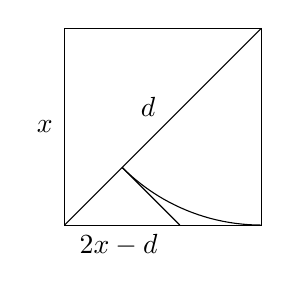
\begin{tikzpicture}[scale=2.5]
  \draw (0, 0) -- (1, 0) -- (1, 1) -- (0, 1) -- cycle;
  \draw[domain=225:270] plot
  ({cos(\x) + 1}, {sin(\x) + 1});

  \draw (45:{sqrt(2) - 1}) --
  ({2 - sqrt(2)}, 0);

  \draw (0, 0) -- (1, 1);

  %\node at (0.8, -0.075) {$d-x$};
  \node at (-0.1, 0.5) {$x$};
  \node at ({0.5-0.075}, 0.6) {$d$};
  % \draw[thick] (0, 0) -- ({2 - sqrt(2)}, 0);
  \node at (0.275, -0.1) {$2x-d$};
\end{tikzpicture}
\end{document}
